
\documentclass[letterpaper, 10 pt, conference]{ieeeconf}  % Comment this line out if you need a4paper
\IEEEoverridecommandlockouts                              % This command is only needed if 
                                                          % you want to use the \thanks command
\overrideIEEEmargins                                      % Needed to meet printer requirements.


% Bibliography
\usepackage{biblatex}
\addbibresource{references.bib}

% Math
\usepackage{physics}
\usepackage{siunitx}
\sisetup{output-exponent-marker=\ensuremath{\mathrm{e}}}
\usepackage{amsmath}
\usepackage{amsfonts}
\usepackage{amssymb}

% Optimization and Algorithms
\usepackage{optidef}
\usepackage{algorithmicx}
\usepackage{algorithm,algpseudocode}

% Formatting
\usepackage{xcolor}
\usepackage{bm}  % for bold symbols 
\usepackage{booktabs}  % better tables
\usepackage{pifont}  % for x mark
\usepackage{graphicx}

% Plotting
\usepackage{pgfplots}
\pgfplotsset{compat=1.15,
	legend style={font=\footnotesize},
}
\usepackage{tikzscale}

% Custom commands
\newcommand{\half}{\frac{1}{2}}
\newcommand{\R}{\mathbb{R}}
\newcommand{\Q}{\mathbb{S}^3}
\newcommand{\skewmat}[1]{[#1]^\times}

\newcommand{\rmap}{\varphi}
\newcommand{\invrmap}{\varphi^{-1}}

\newcommand{\dR}{\delta \mathcal{R}}
\newcommand{\rot}{ \mathcal{R} }
\newcommand{\dq}{\delta q}
\newcommand{\q}{\textbf{q}}
\newcommand{\eq}{_\text{eq}}
\newcommand{\traj}[2][N]{#2_{0:{#1}}}
\newcommand{\pass}{{\color{green} \checkmark}}
\newcommand{\fail}{{\color{red} \ding{55}}}

\newcommand{\todo}[1]{\textcolor{red}{TODO: #1}}


\title{\LARGE \bf
Planning with Attitude
}

\author{Brian Jackson$^1$ and Zachary Manchester$^1$%
    \thanks{
        $^1$Robotics Institute, 
        Carnegie Mellon University, 
        5000 Forbes Ave, Pittsburgh, PA, USA
    }
}

\begin{document}
\maketitle

\section{INTRODUCTION}
    Many useful robotic systems---including quadrotors, airplanes, satellites, autonomous 
    underwater vehicles, and quadrupeds---can perform arbitrarily large three-dimensional 
    translations and rotations as part of their normal operation. 
    While representing translations is straightforward and intuitive, effectively 
    representing the nontrivial group structure of 3D rotations has been a topic of study 
    for many decades. Although we can intuitively deduce that rotations are three-dimensional, 
    a globally non-singular three-parameter representation of the space of rotations does 
    not exist \cite{stuelpnagel1964parametrization}. As a result, when parameterizing rotations, 
    we must either a) pick a three-parameter representation and deal with discontinuities, 
    or b) pick a higher-dimensional representation and deal with constraints between the 
    parameters. While simply representing attitude is nontrivial, generating and tracking 
    motion plans for floating-base systems is an even more challenging problem.
    
    Early work on control problems involving the rotation group dates back to the 1970s, 
    with extensions of linear control theory to spheres \cite{Brockett1973} and $SO(3)$ 
    \cite{Baillieul1978}. Effective attitude tracking controllers have been developed for 
    satellites \cite{wie1985quaternion}, quadrotors \cite{Fresk2013,Liu2015,lee2010geometric,
    Johnson2005,watterson2020control,mellinger2011minimum}, and a 3D inverted pendulum 
    \cite{Chaturvedi2009}  using various methods for calculating three-parameter attitude 
    errors. 
    
    More recently, these ideas have been extended to trajectory generation \cite{Zefran1998}, 
    sample-based motion planning \cite{Zefran1999,Kuffner2004}, and optimal control. 
    Approaches to optimal control on attitude problems include analytical methods applied to
    satellites \cite{Spindler1998}, discrete mechanics \cite{Kobilarov2011,Kobilarov2014,
    Lee2008}, a combination of sampling-based planning and constrained trajectory 
    optimization for satellite formations \cite{Garcia2005, Aoude2008}, projection operators 
    \cite{Saccon2013}, or more general theory for optimization on manifolds 
    \cites{watterson2018trajectory}. 
    Nearly all of these methods rely heavily on principles from differential geometry and 
    Lie group theory; however, despite these works, many recent papers in the robotics 
    community continue to apply traditional methods for motion planning and control with no 
    regard for the group structure of rigid body motion \cite{Alothman2016,deCrousaz2015,
    Williams2017,Geisert2016}.
    
    In this paper, we make a departure from previous approaches to geometric planning and 
    control that rely heavily on ideas and notation from differential geometry, 
    and instead use only basic mathematical tools from linear algebra and calculus that 
    should be familiar to most roboticists. 
    Similar to \cite{Mandic2011,Xu2016}, in Sec. \ref{sec:Quaternion_Calculus} we introduce 
    a quaternion differential calculus, but take a significantly simpler and more general 
    approach that unifies both planning and control, enabling straight-forward adaptation of 
    existing algorithms to systems with quaternion states. 
    To make this concrete, in Sec. \ref{sec:MLQR} we apply our approach to derive an 
    extension to the linear-quadratic regulator (LQR) that we call multiplicative LQR (MLQR), 
    which is the control dual to the multiplicative extended Kalman filter (MEKF) from the 
    state estimation literature \cite{markley2014fundamentals}. 
    In Sec. \ref{sec:experiments} we provide several simulation results demonstrating the 
    application of our method to tracking control and constrained trajectory optimization.
    In summary, our contributions include:

    \begin{itemize}
        \item A unified approach to quaternion differential calculus entirely based on standard vector calculus and linear algebraic operations
        \item Derivation of multiplicative LQR, an adaptation of LQR to the control of systems with quaternion states
        \item A set of benchmark motion-planning and trajectory-tracking problems in which we compare our approach to existing methods commonly used in the robotics community to account for 3D rotations
    \end{itemize}


\section{Background}

    We begin by defining some useful conventions and notation. 
    Attitude is defined as the rotation from the robot's body frame to a global inertial 
        frame. 
    We also define gradients to be row vectors, that is, for 
        $f(x) : \R^n \to \R$, $\pdv{f}{x} \in \R^{1\times n}$.

    \subsection{Unit Quaternions} \label{sec:quaternions}
        We leverage the fact that quaternions are linear operators and that the space of 
        quaternions $\mathbb{H}$ is isomorphic to $\R^4$ to explicitly 
        represent---following the Hamilton convention---a quaternion $\q \in \mathbb{H}$ as 
        a standard vector $q \in \R^4 := [q_s \;\; q_v^T]^T$ where $q_s \in \R$ and 
        $q_v \in \R^3$ are the scalar and vector part of the quaternion, respectively.
        
        Quaternion multiplication is defined as
        \begin{equation} \label{eq:quat_mult}
            \q_2 \otimes \q_1 = L(q_2) q_1 = R(q_1) q_2
        \end{equation}
        where $L(q)$ and $R(q)$ are orthonormal matrices defined as
        \begin{align}
            L(q) &:= \begin{bmatrix} 
                q_s \;\; & -q_v^T \\ 
                q_v \;\; & q_s I + \skewmat{q_v} 
            \end{bmatrix} 
            \label{eq:Lmult} \\
            %= \begin{bmatrix} q & G(q) \end{bmatrix} \label{eq:Lmult} \\
            R(q) &:=\begin{bmatrix} 
                q_s \;\; & -q_v^T \\ 
                q_v \;\; & q_s I - \skewmat{q_v} 
            \end{bmatrix} \label{eq:Rmult},
        \end{align}
        and $\skewmat{x}$ is the skew-symmetric matrix operator
        \begin{equation}
            \skewmat{x} := \begin{bmatrix} 
                0 & -x_3 & x_2 \\ 
                x_3 & 0 & -x_1\\ 
                -x_2 & x_1 & 0 
            \end{bmatrix}.
        \end{equation}
        
        The inverse of a unit quaternion $q^{-1}$, giving the opposite rotation, is equal 
        to its conjugate $q^*$, which is simply the same quaternion with a negated vector 
        part:
        \begin{equation} \label{eq:T}
            \q^* = T q := \begin{bmatrix} 
                1 & \\ 
                & -I_3 
            \end{bmatrix} q
        \end{equation}
        The following identities, which are easily derived from 
        \eqref{eq:Lmult}--\eqref{eq:T}, are extremely useful:
        \begin{align}
            &L(Tq) = L(q)^T = L(q)^{-1} \\
            &R(Tq) = R(q)^T = R(q)^{-1} .
        \end{align}
        
        We will sometimes find it helpful to create a quaternion with zero scalar part from 
        a vector $r \in \R^3$. We denote this operation as,
        \begin{equation}
            \hat{r} = H r \equiv \begin{bmatrix} 0 \\ I_3 \end{bmatrix} r.
        \end{equation}
        Unit quaternions rotate a vector through the operation 
        $\hat{r}' = \q \otimes \hat{r} \otimes \q^*$. 
        This can be equivalently expressed using matrix multiplication as
        \begin{align} 
            r' &= H^T L(q) R(q)^T H r = A(q)r , \label{eq:quaternion_rotation}
        \end{align}
        where $A(q)$ is the rotation matrix in terms of the elements of the quaternion 
        \cite{markley2014fundamentals}. 

    \subsection{Rigid Body Dynamics} \label{sec:rigidbody_dynamics}
        In the current work we will restrict our focus to rigid bodies moving freely in 3D 
        space. That is, we consider systems with dynamics of the following form:
        \begin{equation} \label{eq:rigid_body_dynamics}
            x = \begin{bmatrix} r \\ R \\ v \\ \omega \end{bmatrix}, \quad 
            \dot{x} = \begin{bmatrix} 
                v \\ 
                \texttt{kinematics}(R,\omega) \\ 
                \frac{1}{m} F_G(x,u) \\ 
                J^{-1}(\tau_L(x,u) - \omega \times J \omega) 
            \end{bmatrix}
        \end{equation}
        where $x$ and $u$ are the state and control vectors, $r \in \R^3$ is the position, 
        $R \in SO(3)$ is the attitude, $v \in \R^3$ is the linear velocity, and 
        $\omega \in \R^3$ is the angular velocity. $m \in \R$ is the mass, 
        $J \in \R^{3\times3}$ is the inertia matrix, $F_G(x,u) \in \R^3$ are the forces in the 
        global frame, $\tau_L(x,u)$ are the moments in the local (body) frame, and 
        $\texttt{kinematics}$ are the kinematics for the chosen attitude representation. The 
        kinematics for unit quaternions are
        \begin{equation}
            \dot{q} = \half \q \otimes \hat{\omega} = \half L(q) H \omega.
        \end{equation}

\section{Quaternion Differential Calculus} \label{sec:Quaternion_Calculus}
    We now present a simple but powerful method for taking derivatives of functions 
    involving quaternions based on the notation and linear algebraic operations outlined 
    in Sec. \ref{sec:quaternions}.
    
    \begin{figure}
        \centering
        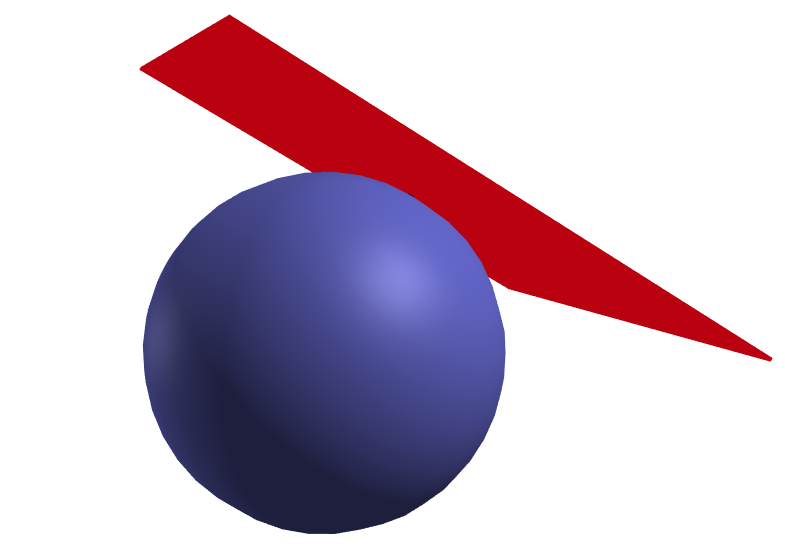
\includegraphics[height=5cm]{figures/tangent_plane.tikz}
        \caption{
            When linearizing about a point $q$ on an sphere $\mathbb{S}^{n-1}$ in 
            n-dimensional space, the tangent space $T$ is a plane living in $\R^{n-1}$, 
            illustrated here with $n=3$. Therefore, when linearizing about a unit 
            quaternion $q \in \Q$, the space of differential rotations lives in $\R^3$.
        }
        \label{fig:tangent_plane}
    \end{figure}
        
        Derivatives consider the effect an infinitesimal perturbation to the input has on
        an infinitesimal perturbation to the output. For vector spaces, the composition
        of the perturbation with the nominal value is simple addition and the
        infinitesimal perturbation lives in the same space as the original vector. For
        unit quaternions, however, neither of these are true; instead, they compose
        according to \eqref{eq:quat_mult}, and infinitesimal unit quaternions are (to
        first order) confined to a 3-dimensional plane tangent to $\Q$ (see Fig.
        \ref{fig:tangent_plane}).

        %, and are related through a non-linear mapping $\varphi : \R^3 \to \Q$ )
        The fact that differential unit quaternions are three-dimensional should make
        intuitive sense: Rotations are inherently three-dimensional and differential
        rotations should live in the same space as angular velocity, i.e. $\R^3$.

        skinny dog runs after skinny cat
        
        There are many possible three-parameter representations for small rotations in
        the literature. Many authors use the exponential map \cite{Baillieul1978,
        Zefran1998, Lee2008, Saccon2013, Sola2017, Fan2016, watterson2018trajectory},
        while others have used the Cayley map (also known as Rodrigues parameters)
        \cite{Kobilarov2011, Kobilarov2014}, Modified Rodrigues Parameters (MRPs)
        \cite{Terzakis2018}, or the vector part of the quaternion \cite{Fresk2013}.
        We choose Rodrigues parameters \cite{markley2014fundamentals} because they are
        computationally efficient and do not inherit the sign ambiguity associated with
        unit quaternions. The mapping between a vector of Rodrigues parameters $\phi \in
        \R^3$ and a unit quaternion $q$ is known as the Cayley map: \begin{equation}
        \label{eq:cayley}
            q = \varphi(\phi) = \frac{1}{\sqrt{1 + \norm{\phi}^2}} \begin{bmatrix} 1 \\ \phi \end{bmatrix}.
        \end{equation}
        We will also make use of the inverse Cayley map:
        \begin{equation}
            \phi = \varphi^{-1}(q) = \frac{q_v}{q_s}.
        \end{equation}

    \subsection{Jacobian of Vector-Valued Functions}
        When taking derivatives with respect to quaternions, we must take into account
        both the composition rule and the nonlinear mapping between the space of unit
        quaternions and our chosen three-parameter error representation.

        Let $\phi \in \R^3$ be a differential rotation applied to a function with
        quaternion inputs $y = h(q): \Q \to \R^p$, such that
        \begin{equation} \label{eq:vector_function}
            y + \delta y = h(L(q) \varphi(\phi)) \approx h(q) +  \nabla h(q) \phi.
        \end{equation}
        We can calculate the Jacobian $\nabla h(q) \in \R^{p \times 3}$ by
        differentiating \eqref{eq:vector_function} with respect to $\phi$, evaluated at
        $\phi = 0$:
        \begin{equation} \label{eq:quat_gradient}
            \nabla h(q) = \pdv{h}{q} L(q) H := \pdv{h}{q} G(q) 
                        = \pdv{h}{q} \begin{bmatrix} 
                            -q_v^T \\ 
                            sI_3 + \skewmat{q_v}
                        \end{bmatrix}
        \end{equation}
        where $G(q) \in \R^{4 \times 3}$ is the \textit{attitude Jacobian}, which
        essentially becomes a ``conversion factor'' allowing us to apply results from
        standard vector calculus to the space of unit quaternions. This form is
        particularly useful in practice since $\pdv*{h}{q} \in \R^{p \times 4}$ can be
        obtained using finite difference or automatic differentiation.
        As an aside, although we have used Rodrigues parameters, $G(q)$ is actually the
        same (up to a constant scaling factor) for any choice of three-parameter attitude
        representation.

    \subsection{Hessian of Scalar-Valued Functions}
	    If the output of $h$ is a scalar ($p = 1$), then we can find its Hessian by
	    taking the Jacobian of \eqref{eq:quat_gradient} with respect to $\phi$ using the
        product rule, again evaluated at $\phi = 0$:

	    \begin{equation} \label{eq:quat_hessian}
            \nabla^2 h(q) = G(q)^T \pdv[2]{h}{q} G(q) + I_3 \pdv{h}{q}q,
	    \end{equation}
	    where the second term comes from the second derivative of $\varphi(\phi)$.
	    Similar to $G(q)$, this ends up being the same (up to a scaling factor) for any
        choice of three-parameter attitude representation.
        
    \subsection{Jacobian of Quaternion-Valued Functions}
        We now consider the case of a function that maps unit quaternions to unit
        quaternions, $q' = f(q) : \Q \to \Q$. Here we must also consider the non-trivial
        effect of a differential value applied to the output, i.e.:
        \begin{equation} \label{eq:dqoutput}
            L(q') \varphi(\phi') = f(L(q)\varphi(\phi)) .
        \end{equation}
        Solving \eqref{eq:dqoutput} for $\phi'$ we find,
        \begin{equation} \label{eq:phiprime}
            \phi' = \varphi^{-1} \left( L(q')^T f(L(q)\varphi(\phi)) \right) \approx \nabla f(q) \, \phi.
        \end{equation}
        Finally, the desired Jacobian is obtained by taking the derivative of
        \eqref{eq:phiprime} with respect to $\phi$:
        \begin{equation} \label{eq:quat_jacobian}
            \nabla f(q) = H^T L(q')^T \pdv{f}{q} L(q) H = G(q')^T \pdv{f}{q} G(q).
        \end{equation}
        The leading $G(q')^T$ comes from the fact that as $\phi' \to 0$, $L(q') f(q) \to
        I_q$, where $I_q$ is the quaternion identity. Differentiating through the inverse
        map, evaluated at the quaternion identity, we find that $\pdv*{\varphi^{-1}}{q}
        \to H^T$ for any three-parameter attitude representation.


\section{Multiplicative LQR} \label{sec:MLQR}
    Leveraging the methods from the previous section, we derive multiplicative LQR
    (MLQR), a variant of LQR that correctly accounts for the group structure of
    rotations. For concreteness, we consider a system with rigid body dynamics, as
    presented in Sec. \ref{sec:rigidbody_dynamics}, and design a controller to stabilize
    the system about a dynamically feasible discretized reference trajectory
    $\bar{x}_{0:N}, \bar{u}_{0:N}$ with $N$ time steps.
    We begin by linearizing the dynamics about the reference trajectory using \eqref{eq:quat_jacobian}. Our linearized error dynamics become
    \begin{equation} \label{eq:linearized_dynamics}
        \delta x_{k+1} = A_k \delta x_k + B_k \delta u_k 
    \end{equation}
    where \begin{equation}
        \begin{aligned}
            A_k = E(\bar{x}_{k+1})^T \pdv{f}{x}|_{\bar{x}_k,\bar{u}_k} E(\bar{x}_k), \\
            B_k = E(\bar{x}_{k+1})^T \pdv{f}{u}|_{\bar{x}_k,\bar{u}_k},
        \end{aligned}
    \end{equation}
    and $\delta x_k \in \R^{12}$ and $E(x_k) \in \R^{12 \times 13}$ are the state error and state error Jacobian:
    \begin{equation} \label{eq:state_error}
        \setlength\arraycolsep{1pt}
        \delta x_k = \begin{bmatrix} 
            r_k - \bar{r}_k \\ \varphi^{-1}(\bar{\q}_k^{-1} \otimes \q_k) \\ v_k - \bar{v}_k \\ \omega_k - \bar{\omega}_k 
        \end{bmatrix}\!, \;
        E(x) = \begin{bmatrix}
            I_3 & & & \\
            & G(q) & & \\
            & & I_3 & \\
            & & & I_3 \\
        \end{bmatrix}\!.
    \end{equation}
    
    With our linearized system, we can apply the traditional LQR Riccati recursion,
    \begin{multline}
         P_k = W_k +  A_k^T P_{k+1} A_k \\
         - A_k^T P_{k+1}^T B_k (R_k + B_k^T P_{k-1} B_k)^{-1} B_k^T P_{k+1} A_k ,
    \end{multline}
    which minimizes the quadratic cost function
    \begin{equation}
        \half \sum_{k=0}^N \delta x_k^T Q_k \delta x_k + \delta u_k^T R_k \delta u_k
    \end{equation}
    of the state \emph{error}, where $Q_k \in \R^{12 \times 12}$ is the weight matrix on
    the state \emph{error}, and $R_k \in \R^m$ is the weight matrix on the controls. From
    this, we get our non-linear feedback policy
    \begin{equation} \label{eq:mlqr_control}
        u = K_k \delta x_k + \bar{u}_k.
    \end{equation}
    where $\delta x_k$ is computed online using the non-linear error function
    \eqref{eq:state_error} and the linear feedback gain $K_k$ is calculated using the
    standard LQR formula:
    \begin{equation} \label{eq:LQR_gain}
         K_k := -(R_k + B_k^T P_{k+1} B_k)^{-1} B_k^T P_{k+1} A_k.
    \end{equation}
    
    The multiplicative Linear Quadratic Regulator is summarized as follows:
    \begin{enumerate}
        \item Pick $Q_k \in \R^{12 \times 12}$ to weight the state \textit{error}, and $R_k \in \R^{m \times m}$
        \item Linearize the dynamics using the state error Jacobian \eqref{eq:state_error}
        \item Compute $K_k$ using the standard LQR Riccati recursion
        \item Online, compute the control using \eqref{eq:state_error} and \eqref{eq:mlqr_control}.
    \end{enumerate}

    \subsection{Constrained Iterative MLQR}
        As demonstrated above, it is very straight-forward to adapt LQR to use
        quaternions. We similarly use this technique to adapt nonlinear trajectory
        optimization algorithms. Here we present the modifications to the ALTRO solver
        \cite{howell2019altro}, which uses iterative LQR (iLQR) combined with an
        augmented Lagrangian approach to handle constraints.
        
        For each iteration of iLQR within ALTRO, we can calculate a quadratic
        approximation of the cost function using \eqref{eq:quat_gradient} and
        \eqref{eq:quat_hessian}. Identical to \eqref{eq:linearized_dynamics}, we use
        \eqref{eq:quat_jacobian} to linearize the dynamics and use MLQR to solve for the
        feedback and feedforward gains.
        
        The only other modification to the algorithm is during the iLQR ``forward pass''
        that simulates the system with the closed-loop MLQR controller, where we use
        \eqref{eq:state_error} to calculate the nonlinear feedback policy during the
        forward roll-outs.
        For robustness, we may also add an additional criterion to the line search that
        checks for singularities in the three-parameter error state which, for the Cayley
        map, occur at \ang{180}, at which point the step size should be reduced.
    
    \subsection{Quaternion Cost Functions} \label{sec:cost_functions}
        In addition to the straight-forward modifications to the LQR algorithm itself, we
        need to carefully consider the types of cost functions we minimize. We frequently
        minimize costs that penalize distance from a goal state, e.g. $\half (x-x_g)^T Q
        (x-x_g)$; however, na\"ive substraction of unit quaternions is ill-defined. We
        propose two different cost functions that accomplish similar behavior.
        For sake of clarity and space, we only consider the costs on the quaternion
        variables: costs on the other states and the control variables remain unaffected.
        
        \subsubsection{Error Quadratic}
            Rather than simple subtraction, we can use a quadratic function on the
            three-parameter error state \eqref{eq:state_error}:
            \begin{equation} \label{eq:error_quadratic}
                J_\text{err} = \half \phi^T Q \phi 
                = \half \left(\varphi^{-1}(\delta q)\right)^T Q 
                        \left(\varphi^{-1}(\delta q)\right).
            \end{equation}
            where $\delta q = L(q_g)^T q$, and $\phi = \varphi{\delta q}$. The gradient
            and Hessian of \eqref{eq:error_quadratic} are
            \begin{equation}
                \nabla J_\text{err }= \phi^T Q  D(\delta q)  G(\delta q)
            \end{equation}
            \begin{equation}
                \begin{aligned}
                     \nabla^2 J_\text{err} &= 
                        G(\delta q)^T \! \left(
                        D(\delta q)^T Q D(\delta q) + \nabla D \right) G(\delta q) 
                      + I_3 (\phi^T Q  D(\delta q)) \delta q %\\
                \end{aligned}
            \end{equation}
            where, for the Cayley map,
            \begin{equation}
                D(q) = \pdv{\varphi^{-1}}{q} = -\frac{1}{q_s^2}\begin{bmatrix}
                    q_v \;\; & -\frac{1}{q_s} I_3
                \end{bmatrix}
            \end{equation}
            \begin{equation}
                \nabla D = \pdv{q}(D(q)^T Q \phi) 
                = -\frac{1}{q_s^2} \begin{bmatrix} 
                    -2 \frac{q_v}{q_s}^T Q \phi & \phi^T Q \\
                                   Q \phi & 0 \\
                \end{bmatrix}.
            \end{equation}

\end{document}